\section{Introduction}\label{sec:introduction}

% Deep neural networks (DNN) led to significant performance improvement in various AI applications, such as speech recognition \cite{RN164,RN165,RN167}, natural language processing \cite{RN168,Luong2015Effective,Wu2016Google}, reinforcement learning \cite{Mnih2013Playing, Mnih2015Human, Silver2016Mastering}, and computer vision (CV). Especially in computer vision, neural networks with convolution as a primary operation, named Convolutional Neural Network (CNN), become the most popular research methods \cite{He2016Deep, RN72,Redmon2016You, Shelhamer2017Fully, Simonyan2014Very}.

% Compared with traditional CV algorithms, neural network algorithms achieve superior performance benefited from the use of larger and deeper models and massive amount of training data~\cite{szegedy2015going, Simonyan2014Very, He2016Deep}. 
Convolutional neural networks (CNN) has made significant performance improvement in computer vision tasks \cite{He2016Deep, Shelhamer2017Fully}. However, the accuracy improvement comes at significant cost of training computation. 
% More and more researchers begin to focus on building efficient models to achieve the best accuracy with a limited model size. 

% In the study of reducing the computational complexity of neural networks, 
Model pruning and quantization have proved to be effective to reduce the requirements of computation, bandwidth and memory footprint, and have almost no effect on the performance (accuracy metric) of neural networks \cite{RN173,RN159,han2015deep}. A series of the hardware accelerator architecture designs are focused on the forward inference phase of neural networks, which takes full advantage of the benefits of sparseness and quantization and shows outstanding performance and energy efficiency. To deploy a sparse network, first the neural network model well-trained in dense needs to be pruned, and the loss of accuracy can be recovered by fine-tuning. Sparse neural networks can be deployed on different platforms and can achieve higher speed and energy efficiency than dense neural networks, as shown in Figure\ref{fig:intro}.

\begin{figure}[htbp]
  \centering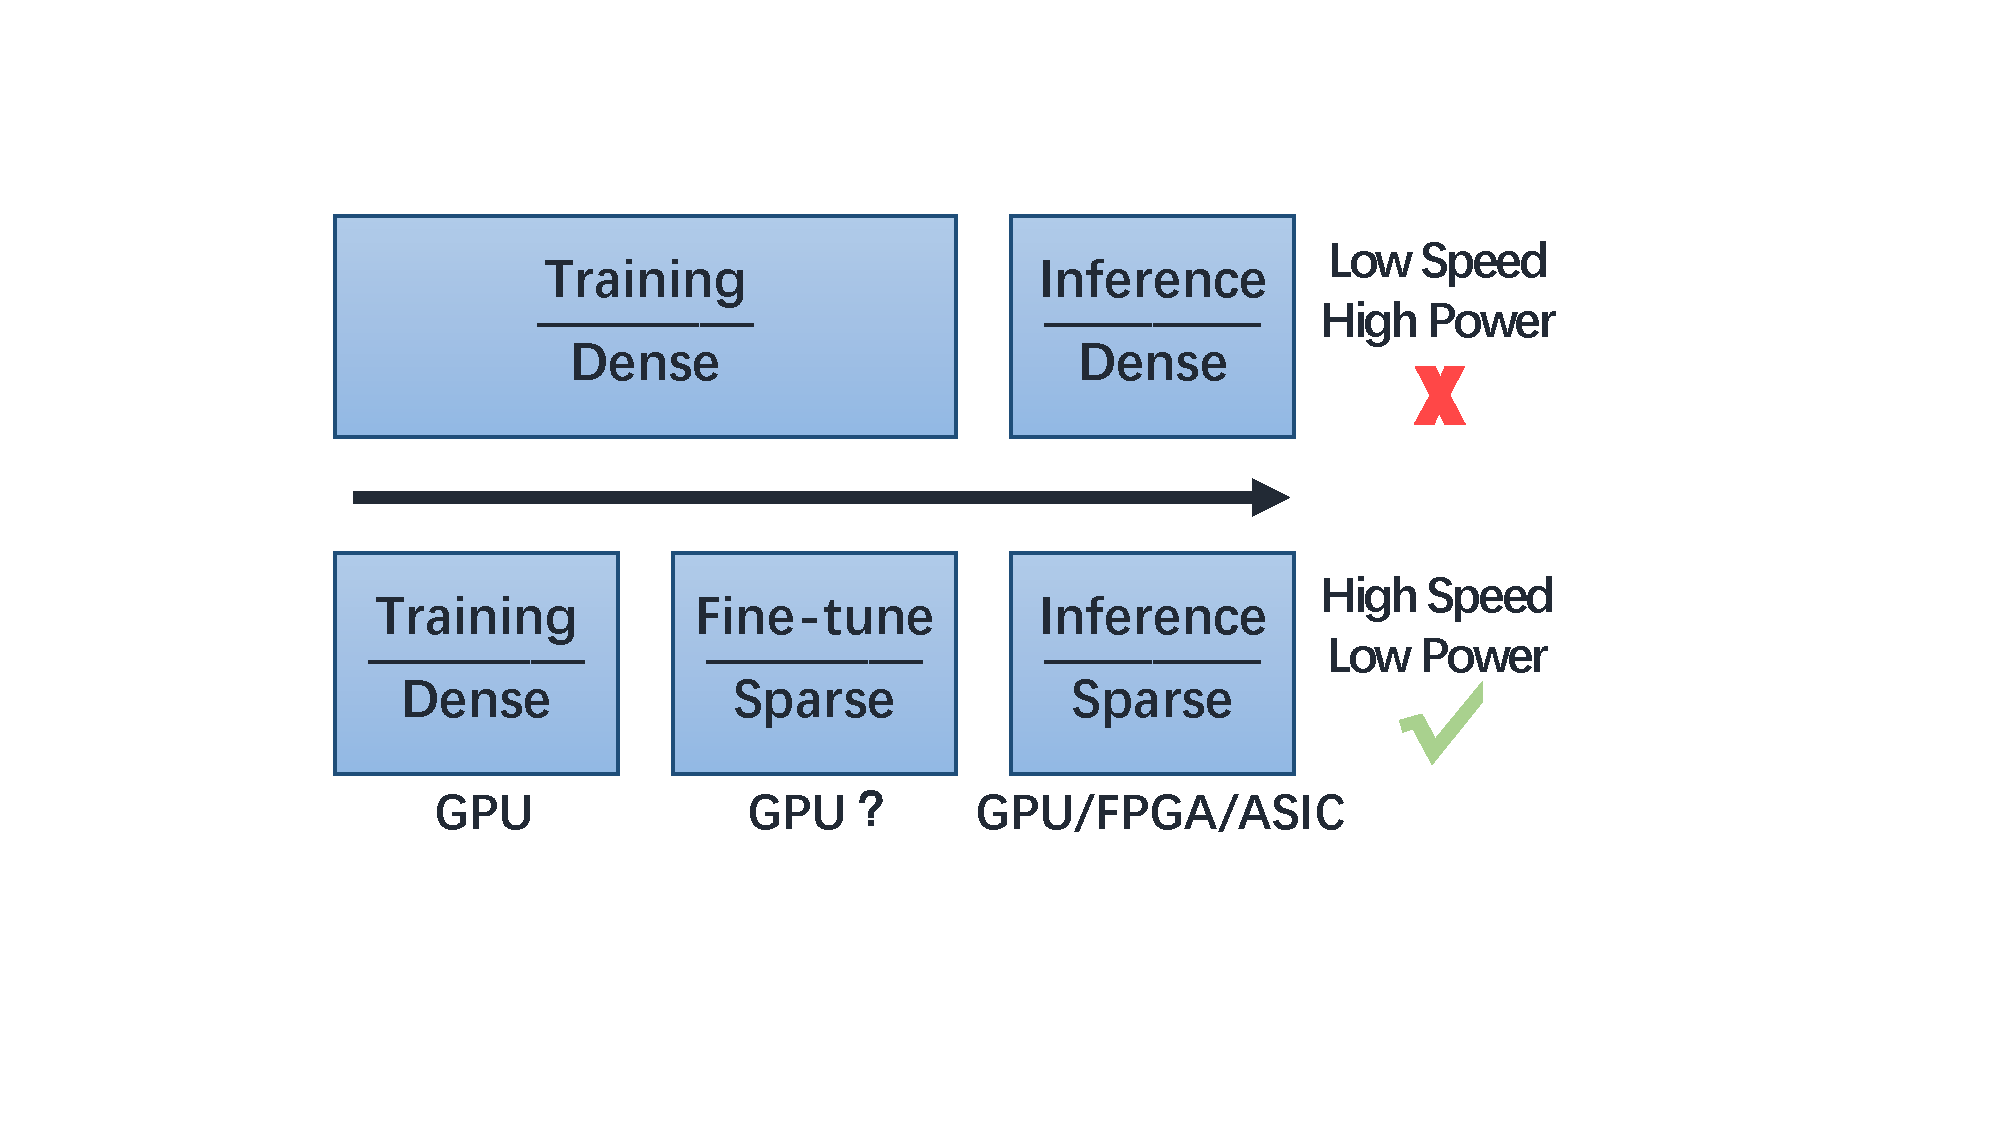
\includegraphics[width=3in]{figures/intro.pdf}
  \caption{Dense training, Sparse fine-tune, Sparse inference}\label{fig:intro}
\end{figure}

Although the GPU is suitable for training of dense neural networks, it can not be a proper user of the sparsity in the sparse neural network to further improve the performance (speed metric). Customized design hardware can make better use of the sparsity of the network to achieve the purpose of improving training efficiency. As a hardware programmable devices, FPGA has been widely deployed in the server cluster \cite{RN169, RN171, RN172}, but there is still no training architecture can take advantage of sparsity. On the other hand, the current fixed-point neural network training algorithm is still not hardware-friendly, for example, need floating point number to calculate the gradients\cite{Zhou2016DoReFa}.

In this paper, we propose an architecture design for sparse neural network training accelerators on the FPGA platform, which reached a high computing capability and energy efficiency. At the same time, we provide a sparse convolution neural network transformation technology, making the sparse neural network more suitable for training and inference on customized hardware platform while maintaining the accuracy at almost the same level. The main contributions of this paper are summarized as follows:
\begin{itemize}
\item A hardware friendly training process is proposed with all-fixed-point operations. 
\item Dedicated processing element (PE) on FPGA is designed to utilize the sparsity in both feed forward and back propagation phases of training.
\item We analyze the limitation on unroll parameters brought by sparsity and loop dimension variety between feed forward and back propagation phases. A corresponding flexible PE array structure is proposed to improve hardware utilization ratio.
\item Data arrangement and schedule strategies are proposed to improve bandwidth utilization .
\end{itemize}
Experimental results show that Proposed hardware achieves 641GOP/s equivalent performance and 3x better energy efficiency compared with GPU. 

The rest of this paper is organized as follows. Section~\ref{sec:preliminary} introduces the background of training of a CNN. Section~\ref{sec:related_work} reviews previous work on software and hardware level CNN optimization. Section~\ref{sec:training} and section~\ref{sec:hw} introduces the proposed training process and hardware platform respectively. Experimental results are shown in section~\ref{sec:experiment}. Section~\ref{sec:conclusion} concludes this paper.
